\documentclass[class=report, crop=false, 12pt,a4paper]{standalone}
\usepackage{enumitem}
\usepackage{multicol}
\usepackage{graphicx}
\usepackage{float}
\usepackage{amsmath}
\usepackage{amssymb}
\usepackage{mathtools}
\usepackage{siunitx}
\usepackage{commath}
\usepackage{array}
\usepackage{natbib}
\usepackage[a4paper,width=150mm,top=25mm,bottom=25mm]{geometry}
\setlength{\parindent}{0pt}
\begin{document}
\section{Failure modes}
Structural failure occurs when a structural component is unable to fulfil its designed purpose. 
\subsection{Forms of failure}
\begin{itemize}
  \item Elastic failure - excessive elastic deformation (e.g. buckling)
  \item Brittle failure - sudden fracture of the component
  \item Plastic failure - permanent variation of geometry
  \item Progressive failure - sudden fracture due to fatigue loading 
  \item Creep - ductile failure due to high loads prolonged in time
  \item Corrosion - loss of surface integrity due to environmental factors
  \item Wearing - loss of surface integrity due to abrasive contact
\end{itemize}
\subsection{Micro-structural failures}
At microscopic level, most forms of mechanical failure occur according to two main mechanisms.
\begin{itemize}
  \item Brittle failure - characterised by the breaking of the atomic bonds
  \item Plastic failure - characterised by the spreading of dislocations through the crystal structure
\end{itemize}
\begin{figure}[H]
  \centering
  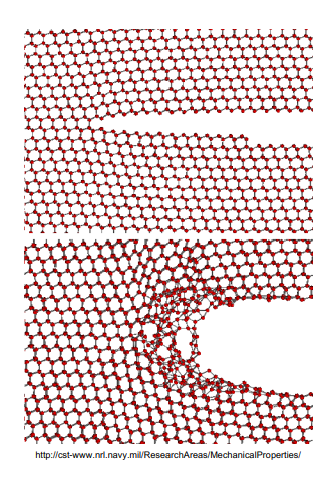
\includegraphics[height = 7cm]{../img/diagram8.png}
  \caption{}
\end{figure}
\textbf{Failure criteria} have the function to give indication on the possibility that one of these mechanisms may occur, for a known state of stress.
\subsection{Ductile and brittle materials}
It is essential, first, to identify which of the two failing mechanisms is going to occur! In static conditions, the selection is simple: it depends essentially on the material subject to the stress state. There are materials that fail according to the brittle failure mechanism in the most of the cases, called \textbf{brittle materials}. There are materials that fail according to the plastic failure mechanism in the most of the cases, called ductile materials. 
\subsection{Brittle materials}
In brittle materials, atoms have low mobility. Failure occurs without visible permanent deformations, when energy is sufficient to break the atomic bonds.
\begin{figure}[H]
  \centering
  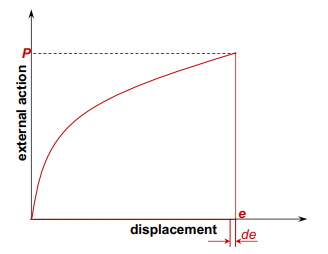
\includegraphics[height = 5cm]{../img/diagram9.png}
  \caption{}
\end{figure}
\subsection{Ductile materials}
In ductile materials, for energy lower than the one producing the spreading of dislocations, atoms undergo reciprocal displacements without breaking atomic bonds: Ductile materials can store large amounts of energy in the form of \textit{recoverable elastic distortion}. This mechanism is called \textbf{elastic behaviour.} For higher levels of energy, dislocations spread and the crystal structure changes. Macroscopically, the component undergoes \textit{permanent deformations}, eventually leading to \textit{fracture.}
\begin{figure}
  \begin{center}
    \begin{minipage}[b]{0.46\textwidth}
      \centering
      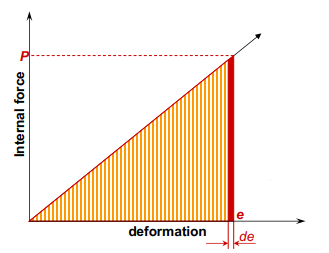
\includegraphics[width = \textwidth]{../img/diagram10.png}
      \caption{}
    \end{minipage}
    \begin{minipage}[b]{0.46\textwidth}
      \centering
      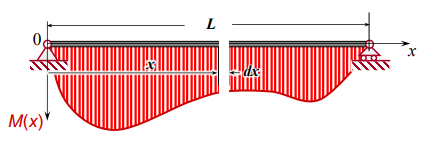
\includegraphics[width = \textwidth]{../img/diagram11.png}
      \caption{}
    \end{minipage}
  \end{center}
\end{figure}
\subsection{Brittle - ductile}
Brittle and ductile materials are only ideal extremes: All materials have an intermediate behaviour. Moreover, under specific states of stress, typically ductile materials can undergo brittle failure and typically brittle materials can fail plastically. 
\begin{figure}[H]
  \centering
  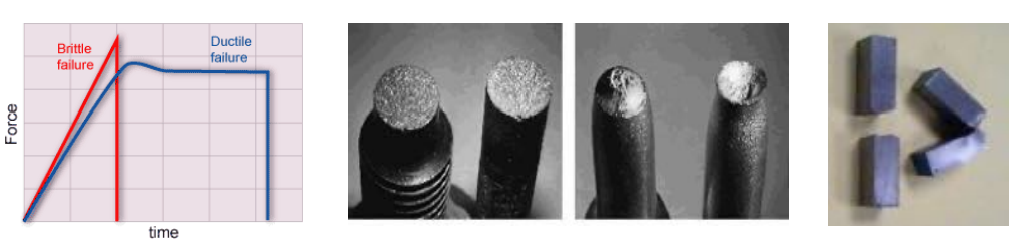
\includegraphics[width = 0.8\textwidth]{../img/diagram12.png}
  \caption{}
\end{figure}
\subsection{Hydrostatic stress state}
\begin{figure}[H]
  \centering
  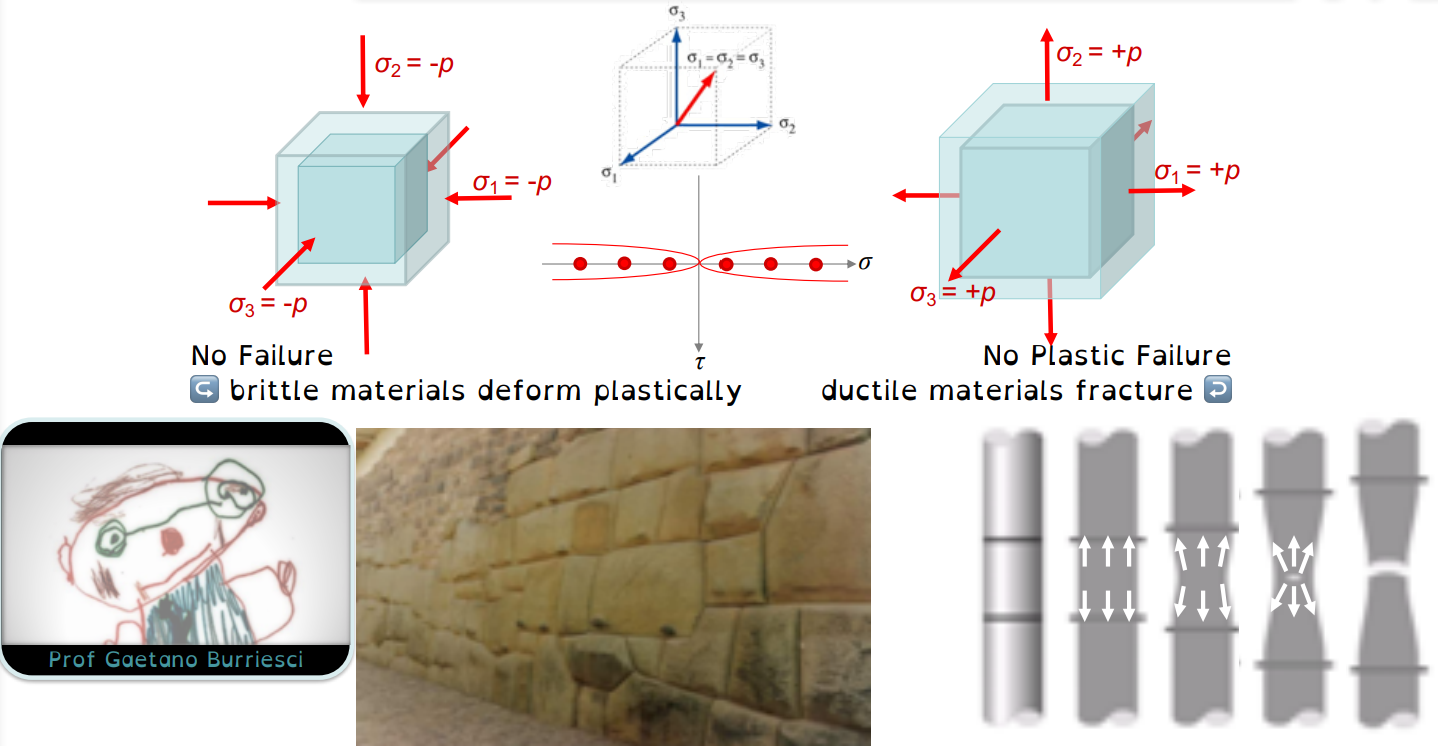
\includegraphics[width =\textwidth]{../img/diagram13.png}
  \caption{}
\end{figure}
\section{Failure criteria}
Experience has shown that failure consistently occurs when the \textit{components of the stress tensor} at a point of the structure reach specific values, depending on the \textit{material}. The state of stress can be easily determined analytically or numerically. However, since infinite different states of stress can occur, \textit{it is impossible to analyse what is the limiting level for all cases.} A possible solution would be to convert a specific state of stress into a single equivalent scalar value, called \textbf{effective stress}, which can represent it and can be  directly compared with a limit value, associated with failure.
\begin{quotation}
  Failure criteria suggest \textbf{how to combine the components of a specific state to obtain an effective stress}.
\end{quotation}
Once the appropriate failure criterion has been identified, the \textit{limit for the effective stress} can be easily measured by determining when failure occurs in a simplified case, e.g. unidirectional tensile or compressive test.
\begin{figure}[H]
  \centering
  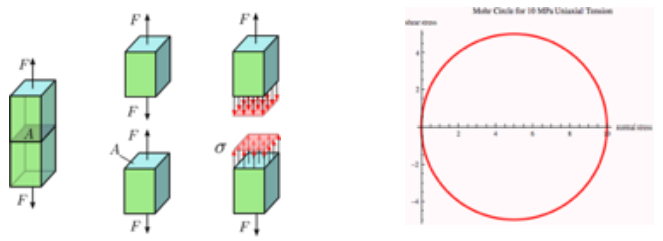
\includegraphics[width = 0.6\textwidth]{../img/diagram14.png}
  \caption{}
\end{figure}
For ductile materials, failure is commonly associated with yielding. For brittle materials it is associated with brittle fracture. 
\section{Maximum principal stress theory}
The first failure criterion can be attributed to Galileo Galilei who observed (from the studies on stone ties) that there is a limit to the maximum principal stress. 
\begin{quotation}
  \textbf{Failure occurs whenever the maximum principal stress equals the strength of the material.}
\end{quotation}
The structure is safe if at all points it is:
\begin{equation}
  \sigma_1 < \sigma_f \, \& \, \sigma_2 < \sigma_f \, \& \, \sigma_3 < \sigma_f
\end{equation}
\subsection{Max \& min principal stress theory}
The \textit{maximum and minimum principal stress theory,} usually attributed to Rankine, includes in the previous criterion a limit to the compressive stress.
\begin{quotation}
  \textbf{Failure occurs whenever the maximum principal stress equals the tensile strength or the minimum principal stress equals the compressive strength.}
\end{quotation} 
\begin{equation}
  \sigma_{fc} < \sigma_1 < \sigma_{ft} \, \& \, \sigma_{fc} < \sigma_2 < \sigma_{ft} \, \& \, \sigma_{fc} < \sigma_3 < \sigma_{ft} 
\end{equation}
Representing the points of safety in a plane $\sigma_1$, $\sigma_2$, a square is described. Representing the points of safety in a space $\sigma_1$, $\sigma_2$, $\sigma_3$, a cube is described.
\begin{figure}
  \begin{center}
    \begin{minipage}[b]{0.46\textwidth}
      \centering
      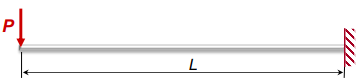
\includegraphics[width = \textwidth]{../img/diagram15.png}
      \caption{}
    \end{minipage}
    \begin{minipage}[b]{0.46\textwidth}
      \centering
      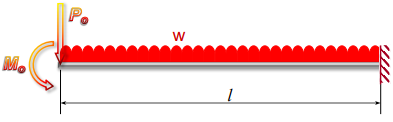
\includegraphics[width = \textwidth]{../img/diagram16.png}
      \caption{}
    \end{minipage}
  \end{center}
\end{figure}
In the Mohr's representation, all circles between two vertical lines of abscissas $\sigma_{ft}$ and $\sigma_{fc}$ described safe states of stress.
\begin{figure}[H]
  \centering
  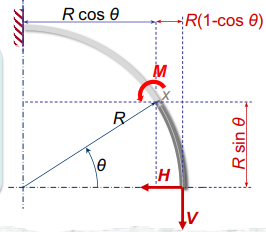
\includegraphics[height = 7cm]{../img/diagram17.png}
  \caption{}
\end{figure}
The main limitations of the maximum principle stress theory are:
\begin{itemize}
  \item interaction between the principal stress is not considered
  \item does not predict unlimited resistance under hydrostatic compression. 
\end{itemize}
Applicability:
\begin{quotation}
  \textbf{The maximum principal stress theory can be reliable only for the study of brittle materials subjected to states of stress different from the hydrostatic compression.}
\end{quotation}
\subsection{Maximum normal strain theory}
The \textit{maximum normal strain theory}, usually attributed to Saint-Venant, is conceptually different, in that it limits the strain instead of the stress. It was developed to justify the vertical cracks that break stone columns.
\begin{quotation}
  \textbf{Failure occurs whenever the maximum principal strain equals the strain corresponding to the tensile strength.}
\end{quotation}
The structure is safe if at all points it is:
\begin{equation}
  \epsilon_1 < \epsilon_f ; \, \epsilon_2 < \epsilon_f ; \, \epsilon_3 < \epsilon_f
\end{equation}
Since:
\begin{align}
  \epsilon_1 &= \frac{1}{E} \left[\sigma_1 - \nu \left(\sigma_2 + \sigma_3\right)\right]\\
  \epsilon_1 &= \frac{1}{E} \left[\sigma_2 - \nu \left(\sigma_1 + \sigma_3\right)\right]\\
  \epsilon_1 &= \frac{1}{E} \left[\sigma_3 - \nu \left(\sigma_1 + \sigma_2\right)\right]
\end{align}
and, from a uni-axial tensile test:
\begin{equation}
  \epsilon_f = \frac{\sigma_f}{E}
\end{equation}
We can derive that:
\begin{align}
  \sigma_1 - \nu \left(\sigma_2 + \sigma_3\right) &< \sigma_f\\
  \sigma_2 - \nu \left(\sigma_1 + \sigma_3\right) &< \sigma_f\\
  \sigma_3 - \nu \left(\sigma_1 + \sigma_2\right) &< \sigma_f
\end{align}
Representing the points of safety in the plane $\sigma_1$, $\sigma_2$, a triangle is obtained. Representing the points of safety in a space $\sigma_1$, $\sigma_2$, $\sigma_3$, a pyramid of triangular equilateral section is obtained.
\begin{figure}
  \begin{center}
    \begin{minipage}[b]{0.46\textwidth}
      \centering
      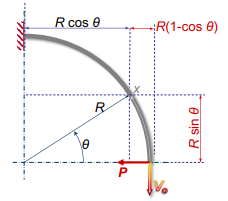
\includegraphics[width = \textwidth]{../img/diagram18.png}
      \caption{}
    \end{minipage}
    \begin{minipage}[b]{0.46\textwidth}
      \centering
      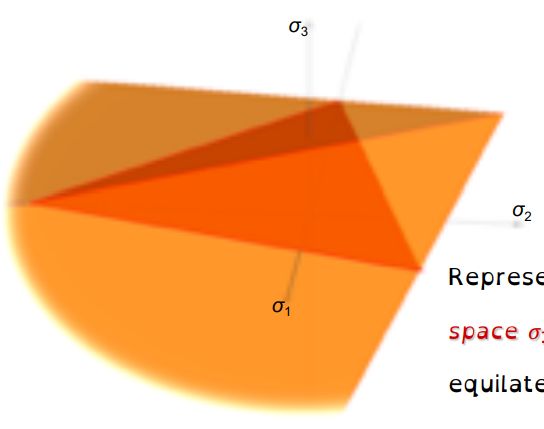
\includegraphics[width = \textwidth]{../img/diagram19.png}
      \caption{}
    \end{minipage}
  \end{center}
\end{figure}
The \textit{maximum normal strain theory} was completed by Grashof, who introduced a limit to the maximum negative strain also. The main limitations of the maximum strain theory are:
\begin{itemize}
  \item though very used in the past, it does not give results in agreement with experimental evidence
  \item does not predict unlimited resistance under hydrostatic compression.
\end{itemize}
Applicability:
\begin{quotation}
  \textbf{the maximum normal strain theory is reliable for the stufy of brittle materials with tensile and compressive strengths not very different, subjected to states of stress different from the hydrostatic compression.}
\end{quotation}
It was the first principle to consider the interaction between principal stresses.
\section{Maximum shear stress theory}
\subsection{Criteria for ductile materials}
Previous criteria were developed when the materials of main interest were brittle (stones, bricks and timbers); and therefore they are suitable to describe brittle failure. When the use of metals became more relevant, new criteria had to be developed, in order to better describe the ductile failure due to yielding. 
\begin{figure}
  \begin{center}
    \begin{minipage}[b]{0.46\textwidth}
      \centering
      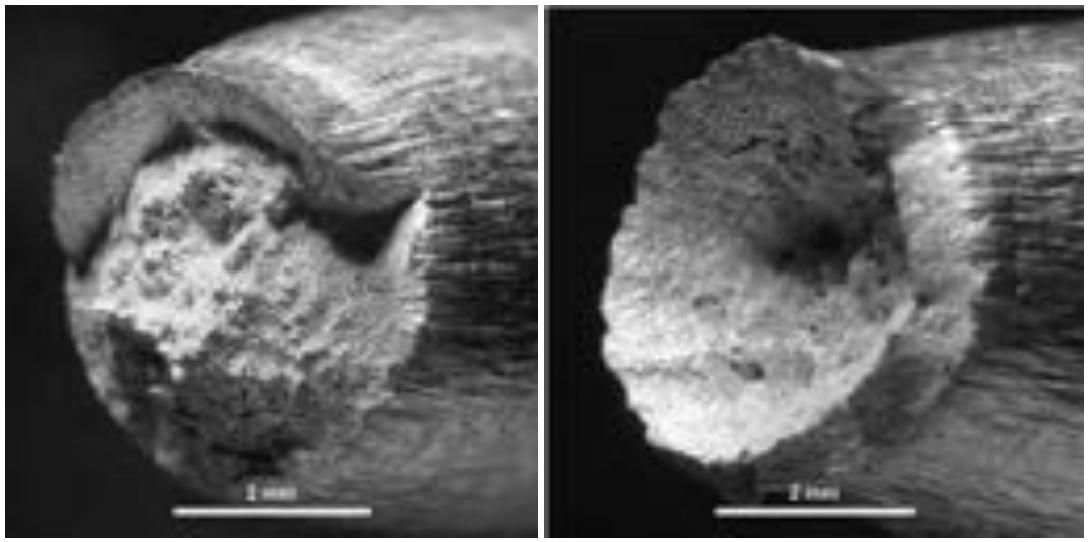
\includegraphics[width = \textwidth]{../img/diagram20.png}
      \caption{}
    \end{minipage}
    \begin{minipage}[b]{0.46\textwidth}
      \centering
      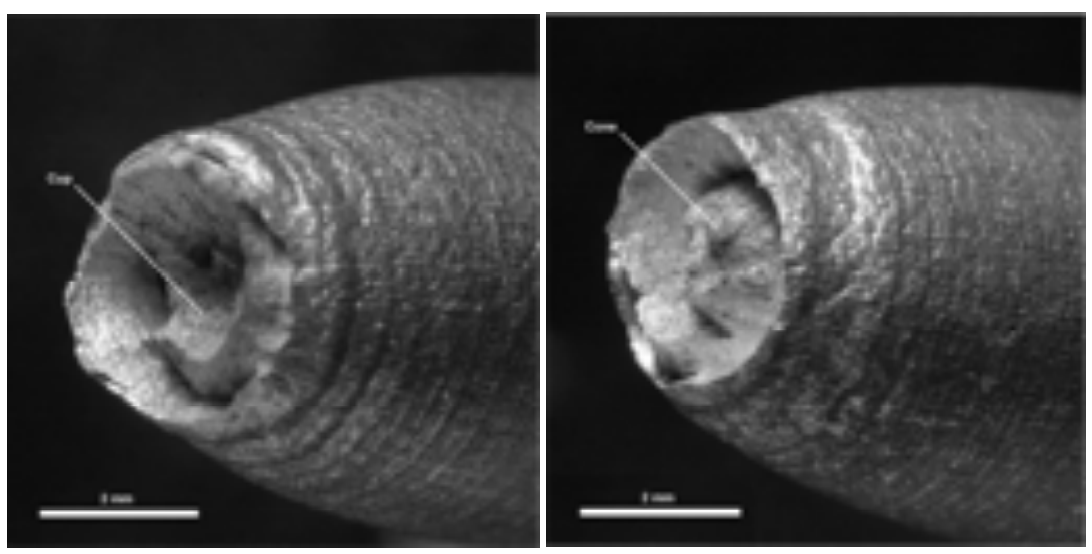
\includegraphics[width = \textwidth]{../img/diagram21.png}
      \caption{}
    \end{minipage}
  \end{center}
\end{figure}
The maximum-shear-stress theory (also called Tresca theory) assumes that plastic failure (yielding) is produced by the shear stresses. 
\begin{quotation}
  \textbf{Yielding occurs whenever the maximum shear stress equals the maximum shear stress $\tau_y$ produced in a tension-test specimen of the same material when that specimen begins to yield.}
\end{quotation}
The structure is safe if at all points it is:
\begin{equation}
  \tau_{max} < \tau_Y
\end{equation}
The maximum shear stress $\tau_Y$ produced in a tension-test specimen when that specimens begins to yield is given by:
\begin{equation}
  \tau_Y = \frac{1}{2}\sigma_Y
\end{equation}
\begin{figure}
  \begin{center}
    \begin{minipage}[b]{0.46\textwidth}
      \centering
      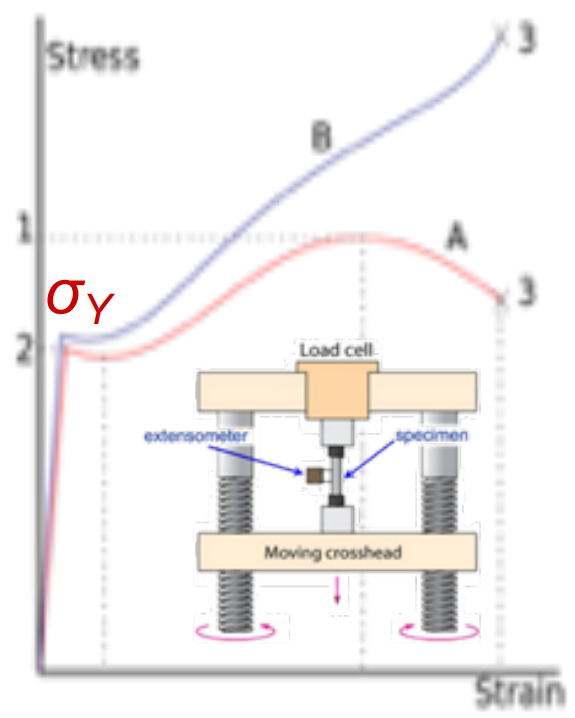
\includegraphics[width = 0.8 \textwidth]{../img/diagram22.png}
      \caption{}
    \end{minipage}
    \begin{minipage}[b]{0.46\textwidth}
      \centering
      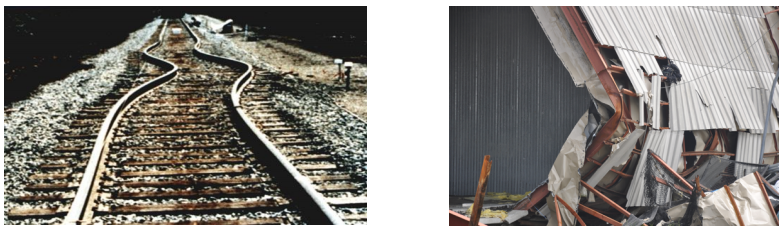
\includegraphics[width = 0.8\textwidth]{../img/diagram23.png}
      \caption{}
    \end{minipage}
  \end{center}
\end{figure}
Maximum shear stresses in the principal planes of the component will be the maximum of:
\begin{equation}
  \left(\tau_{max}\right)_3 = \frac{\left| \sigma_1 - \sigma_2 \right| }{2} \ \left(\tau_{max}\right)_1 = \frac{\left| \sigma_2 - \sigma_3 \right| }{2} \ \left(\tau_{max}\right)_2 = \frac{\left| \sigma_3 - \sigma_1 \right| }{2} 
\end{equation}
\begin{figure}[H]
  \centering
  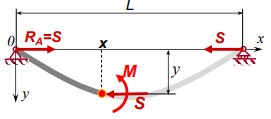
\includegraphics[height = 5cm]{../img/diagram24.png}
  \caption{}
\end{figure}
Therefore:
\begin{equation}
  \left| \sigma_1 - \sigma_2 \right| ; \, \left| \sigma_2 - \sigma_3 \right| ; \, \left| \sigma_3 - \sigma_1 \right| < \sigma_Y
\end{equation}
For a plane stress state $\left(\sigma_3 = 0\right)$:
\begin{equation}
  \tau_{max} < \tau_Y \rightarrow \left| \sigma_1 - \sigma_2 \right| ; \, \left| \sigma_2 - \sigma_3 \right| ; \, \left| \sigma_3 - \sigma_1 \right| < \sigma_Y
\end{equation}
\begin{align}
  \left| \sigma_1 - \sigma_2 \right| < \sigma_Y &\rightarrow \begin{array}{l}
    \sigma_2 - \sigma_Y < \sigma_1 < \sigma_2 + \sigma_Y\\
    \sigma_1 - \sigma_Y < \sigma_2 < \sigma_1 + \sigma_Y
  \end{array}\\
  \left| \sigma_2 \right| < \sigma_Y &\rightarrow - \sigma_Y < \sigma_2 < \sigma_Y\\
  \left| \sigma_1 \right| < \sigma_Y &\rightarrow - \sigma_Y < \sigma_1 < \sigma_Y
\end{align}
An irregular hexagon is described.
\begin{figure}[H]
  \centering
  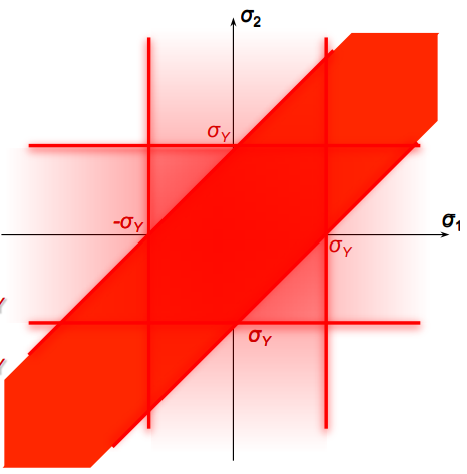
\includegraphics[height = 5cm]{../img/diagram25.png}
  \caption{}
\end{figure}
For a tri-axial stress state:
\begin{equation}
  \tau_{max} < \tau_Y \rightarrow \left| \sigma_1 - \sigma_2 \right| ; \, \left| \sigma_2 - \sigma_3 \right| ; \, \left| \sigma_3 - \sigma_1 \right| < \sigma_Y
\end{equation}
Representing the points of safety in a space $\sigma_1$, $\sigma_2$, $\sigma_3$, a prism of regular hexagonal section, with axis along the trisector to the planes is described.
\begin{figure}[H]
  \centering
  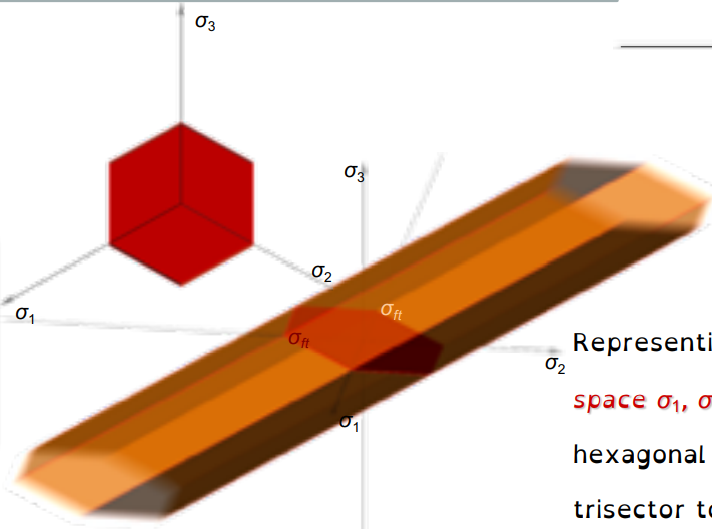
\includegraphics[height = 5cm]{../img/diagram26.png}
  \caption{}
\end{figure}
In the Mohr's representation, all circles between the two horizontal lines of ordinate $\frac{1}{2}\sigma_Y$ and $-\frac{1}{2}\sigma_Y$ describe the safe state of stress.
\begin{figure}[H]
  \centering
  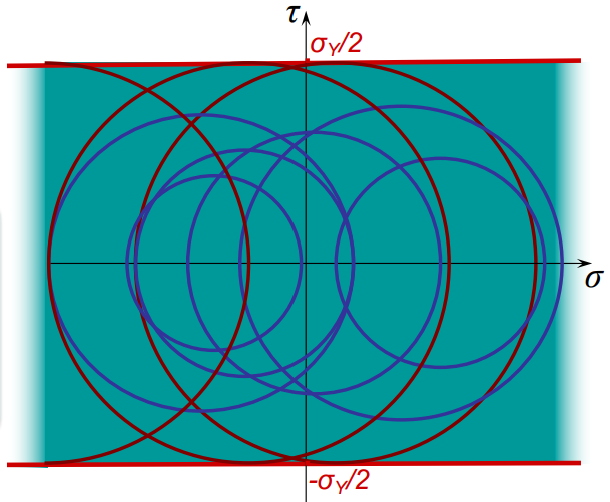
\includegraphics[height = 5cm]{../img/diagram27.png}
  \caption{}
\end{figure}
Applicability:
\begin{quotation}
  \textbf{The maximum shear stress theory is reliable for the study of ductile materials. For these material it is conservative (does not consider the benefit given by the intermediate principal stress). It does not limit hydrostatic compressive loads (in agreement with experimental evidence).}
\end{quotation}
The main limitation of the maximum shear stress theory is that it does not predict the failure under hydrostatic tension.
\section{Maximum energy theories}
\subsection{Maximum strain energy theory}
The criterion proposed by Beltrami assumes that a material can store a limited amount of elastic energy as strain before undergoing plastic deformations (failure).
\begin{quotation}
  \textbf{Yielding occurs whenever the strain energy density equals the strain energy density that produces yielding in a tension-test specimen of the same material.}
\end{quotation}
\begin{align}
  \frac{\dif W}{\dif V} &= \frac{1}{2} \left( \sigma_1 \cdot \epsilon_1 + \sigma_2 \cdot \epsilon_2 + \sigma_3 \cdot \epsilon_3 \right)\\
  &= \frac{1}{2E} \left[ \sigma_1^2 + \sigma_2^2 - 2\nu\left(\sigma_1 \cdot \sigma_2 + \sigma_2 \cdot \sigma_3 + \sigma_3 \cdot \sigma_1 \right) \right]
\end{align}
\begin{equation}
  \begin{array}{l}
    \epsilon_1 = \frac{1}{E} \left[\sigma_1 - \nu \left(\sigma_2 + \sigma_3\right)\right]\\
    \epsilon_1 = \frac{1}{E} \left[\sigma_2 - \nu \left(\sigma_1 + \sigma_3\right)\right]\\
    \epsilon_1 = \frac{1}{E} \left[\sigma_3 - \nu \left(\sigma_1 + \sigma_2\right)\right]
  \end{array} \textrm{ and } \frac{\dif W_Y}{\dif V} = \frac{1}{2} \sigma_Y \cdot \epsilon_Y = \frac{1}{2}\sigma_Y \cdot \frac{\sigma_Y}{E}
\end{equation}
\begin{equation}
  \sigma_1^2 + \sigma_2^2 + \sigma_3^2 - 2\nu \left(\sigma_1 \cdot \sigma_2 + \sigma_2 \cdot \sigma_3 + \sigma_3 \cdot \sigma_1 \right) < \sigma_Y^2
\end{equation}
\begin{figure}[H]
  \centering
  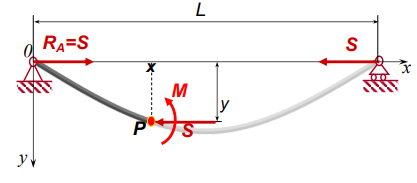
\includegraphics[height = 5cm]{../img/diagram28.png}
  \caption{}
\end{figure}
Representing the points of safety in a plane $\sigma_1$, $\sigma_2$, $\sigma_3 = 0$, an ellipse is described. Representing the points of safety in a space $\sigma_1$, $\sigma_2$, $\sigma_3$, an axial-symmetric ellipsoid with an axis along the trisector to the planes is described.
\begin{figure}
  \begin{center}
    \begin{minipage}[b]{0.46\textwidth}
      \centering
      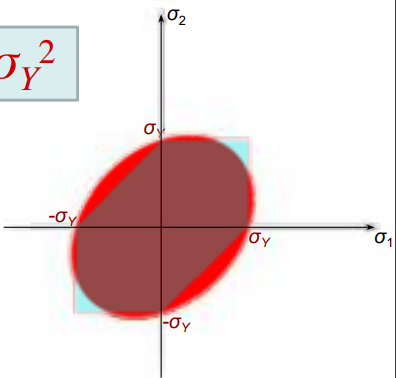
\includegraphics[width = \textwidth]{../img/diagram29.png}
      \caption{}
    \end{minipage}
    \begin{minipage}[b]{0.46\textwidth}
      \centering
      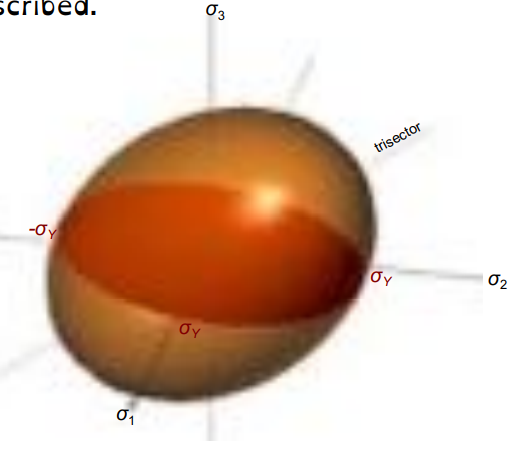
\includegraphics[width = \textwidth]{../img/diagram30.png}
      \caption{}
    \end{minipage}
  \end{center}
\end{figure}
Applicability:
\begin{quotation}
  \textbf{The maximum strain energy theory can be used for the study of ductile materials. It is usually very conservative, especially close the hydrostatic states of stress.}
\end{quotation}
It was the first principle based on energetic considerations.
\end{document}